\newprob{1718626986}
{
    % Active physics p184 7
    下圖顯示一矩形變化的交變電流。其方均根值是 多少?
    \par{\par\centering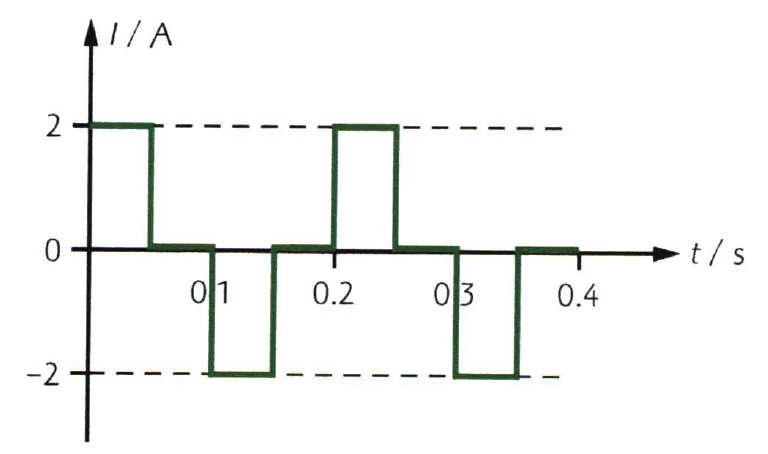
\includegraphics[width=.4\textwidth]{./img/ch_ACtransformer_mc_2024-06-17-20-23-17.png}\par}
    \begin{tasks}
        \task $\dfrac{1}{\sqrt{2}}\unit{A}$
        \task $1\unit{A}$
        \task $\sqrt{2}\unit{A}$
        \task $2\unit{A}$
    \end{tasks}
}{C}

\newprob{1718627097}
{
    % Active physics p184 8
    以左圖的正弦電壓 $V_1$ 加於電阻器 $R$,電阻器會發 熱,平均放熱率為$W$。若改以右圖的方波電壓$V_2$ 加於電阻器 $R$,問平均放熱率為多少?
    \par{\par\centering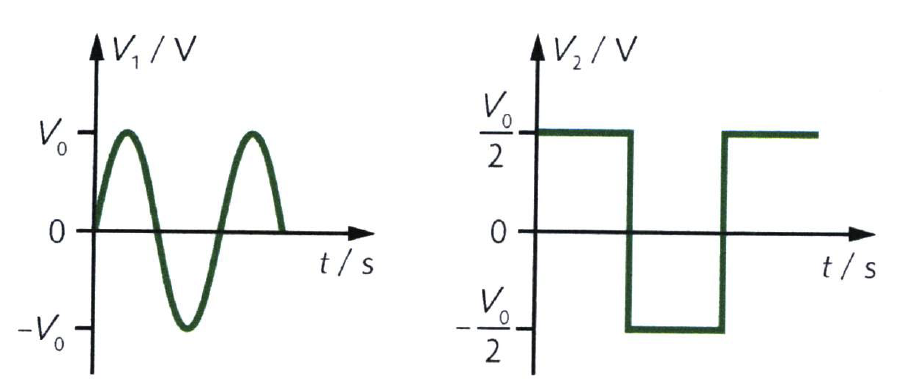
\includegraphics[width=.65\textwidth]{./img/ch_ACtransformer_mc_2024-06-17-20-25-50.png}\par}
    \begin{tasks}
        \task $W/2$
        \task $W/\sqrt{2}$
        \task $W$
        \task $2W$
    \end{tasks}
}{A}

\newprob{1718611244}
{
    % Active physics p330 q1
    為甚麼使用交流電而非直流電來輸電?
    \begin{tasks}
        \task 交流電路較安全。
        \task 交流電壓易於提升和降低。
        \task 交流電功率易於提升。
        \task 輸電過程損失較少能量。
    \end{tasks}

}{
    B
}

\newprob{1718626213}
{
    % Active physics p330 q2
    由於發電廠一般遠離民居興建,因此便要倚賴輸 電纜把電力輸送至客戶。若發電廠生產的電能以 電勢$V$ 和電流$I$,通過電阻為$R$的輸電纜輸送, 輸電纜上的耗電功率為多少?
    \begin{tasks}
        \task 0
        \task $VI$
        \task $I^2R$
        \task $V^2/R$
    \end{tasks}

}{C}

\newprob{1718626292}
{
    % Active physics p330 q3
    為減少功率損失,電力以高電壓輸送,也就是 說,在電網系統中,哪兩點的電勢差最大?
    \par{\par\centering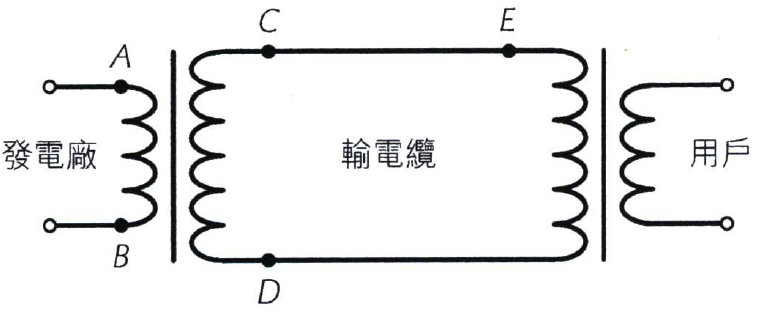
\includegraphics[width=.35\textwidth]{./img/ch_ACtransformer_mc_2024-06-17-20-11-50.png}\par}
    \begin{tasks}
        \task $A$ 和 $B$
        \task $C$ 和 $D$
        \task $C$ 和 $E$
        \task 以上各個選項的電勢差都相同。
    \end{tasks}
}{B}

\newprob{1718626356}
{
    % Active physics p334 q7
    考慮以下方程:
    \begin{align*}
        \frac{\textrm{副電壓}}{\textrm{原電壓}} = \frac{\textrm{副線圈匝數}}{\textrm{原線圈匝數}}
    \end{align*}
    在下列哪些情況中,以上關係\textbf{並不}適用?
    \begin{statements}
        \task 軟鐵心中有磁通量漏失。
        \task 副線圈連接至斷路。
        \task 原線圈與副線圈的電阻不可忍略。
    \end{statements}
    \begin{tasks}
        \task 只有(1)和(2)
        \task 只有(1)和(3)
        \task 只有(2)和(3)
        \task (1), (2) 和 (3)
    \end{tasks}
}{
    B
    (注意線圈電壓在非理想情況下,不一定等於電動勢)
}

\newprob{1718626835}
{
    % Active physics p334 q8
    完全相同的燈泡$X$和$Y$連接至一個變壓器,如 圖。起初,開關$S$斷開。
    \par{\par\centering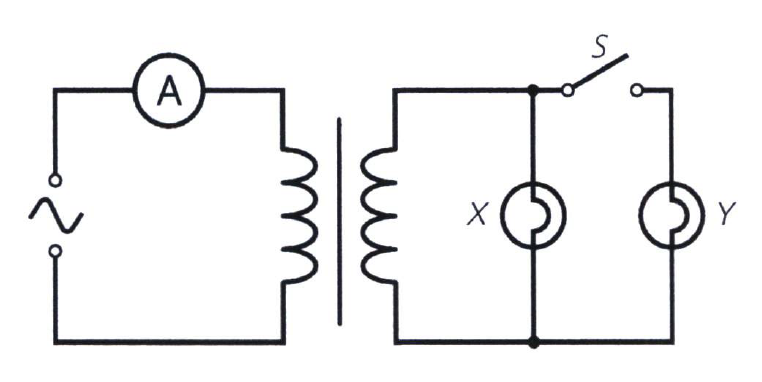
\includegraphics[width=.5\textwidth]{./img/ch_ACtransformer_mc_2024-06-17-20-21-05.png}\par}
    現把開關$S$合上。哪些敘述是正確的?
    \begin{statements}
        \task 燈泡$X$的亮度不變。
        \task 變壓器的效率增倍。
        \task 通過安培計的電流增倍。
    \end{statements}
    \begin{tasks}
        \task 只有(1)
        \task 只有(1)和(3)
        \task 只有(2)和(3)
        \task (1), (2) 和 (3)
    \end{tasks}
}{B}